\section{Efficiency Evaluation \& Simulations}
  \label{section:comparison}
  We offer here a cost and efficiency comparison of this work with
  LVPC~\cite{10.1007/978-3-030-65411-5_18} and Donner~\cite{donner}. We focus on
  these because they are the only ones that enable
  virtual channels over any number of base channels. We remind that LVPC
  achieves this via its recursive property, while Donner
  because it is variadic (c.f.\ Table~\ref{table:comparison-features}).

  We first count the communication, storage and on-chain cost of a virtual
  channel under each protocol. We then simulate the execution of a large number
  of payments among many parties and derive payment latency and fees. We thus
  obtain an end-to-end understanding of both the requirements and the benefits
  each protocol provides.

  \paragraph{Cost calculation.} We consider the general $n$-party case: $1$
  funder ($P_1$), $1$ fundee ($P_n$) and $n-2$ intermediaries ($P_2, \dots,
  P_{n-1}$) where each party has one base channel with each adjacent party. Our
  comparison regards the off-chain cost of opening
  (Table~\ref{table:comparison:overhead:n-parties:open}) and the on-chain cost
  of unilaterally closing
  (Table~\ref{table:comparison:overhead:n-parties:close}).

  Regarding channel opening, in
  Table~\ref{table:comparison:overhead:n-parties:open} we measure for each of
  the three protocols the number of communication rounds required, the total
  size of the outgoing messages as well as the amount of space for storing
  channel data. We measure from the perspective of the funder, the fundee
  and an intermediary, along with the aggregate for all parties.

  % splncs
  %\addtolength{\intextsep}{-30pt}
  \begin{table*}[h!]
    \resizebox{\textwidth}{!}{%
    \begin{tabular}{|l|c|c|c|c|c|c|c|c|c|c|c|}
    \hline
    \multicolumn{12}{|c|}{Open} \\
    \hline
    \multirow{3}{*}{}
              & \multicolumn{3}{|c|}{Funder} & \multicolumn{3}{|c|}{Fundee}
              & \multicolumn{3}{|c|}{Intermediary}
              & \multicolumn{2}{|c|}{Total} \\
    \cline{2-12}
              & \multirow{2}{*}{\shortstack{party \\ rounds}}
              & \multicolumn{2}{|c|}{size} & \multirow{2}{*}{\shortstack{party
              \\ rounds}} & \multicolumn{2}{|c|}{size}
              & \multirow{2}{*}{\shortstack{party \\ rounds}}
              & \multicolumn{2}{|c|}{size} & \multicolumn{2}{|c|}{size} \\
    \cline{3-4} \cline{6-7} \cline{9-12}
              & & sent & stored & & sent & stored & & sent & stored & sent &
              stored \\
    \hline
    LVPC      & $8(n-2)$ & $1381(n-2)$ & $3005(n-2)$ & $7$ & $1254$ & $2936$
              & $16$ & $2989$ & $6385$ & $4370n-8740$ & $9390n-18780$ \\
    \hline
    % my count
    %Donner     & $2$ & $164n + 1934$ & $108n + 2150$ & $1$ & $44n+128$
    %           & $176n+496$ & $1$ & $76n + 2010$ & $132n+2370$
    %           & $132n^2+2390n-2094$ & $76n^2+2066n-1858$ \\
    %\hline
    \multirow{2}{*}{Donner}
              & \multirow{2}{*}{$2$} & \multirow{2}{*}{$184n + 829$}
              & \multirow{2}{*}{\shortstack{$1332.5k+$ \\ $43n+125.5$}}
              & \multirow{2}{*}{$1$} & \multirow{2}{*}{$43n+192.5$}
              & \multirow{2}{*}{\shortstack{$1332.5k+$ \\ $43n+125.5$}}
              & \multirow{2}{*}{$1$} & \multirow{2}{*}{$547$}
              & \multirow{2}{*}{\shortstack{$1332.5k+$ \\ $43n+125.5$}}
              & \multirow{2}{*}{$774n-71$}
              & \multirow{2}{*}{\shortstack{$1332.5kn +$ \\ $43n^2 + 125.5n$}}
              \\
              & & & & & & & & & & & \\
              % For Donner, I drew the storage numbers from
              % https://eprint.iacr.org/2021/855.pdf, p. 22. I'm not sure what
              % pid is, so these numbers may have to be revised.
    \hline
    \multirow{3}{*}{Elmo}
              & \multirow{3}{*}{$6$} &
              \multirow{3}{*}{\shortstack{$32n^3-128n^2$ \\
              $+544n-276$}} &
              \multirow{3}{*}{\shortstack{$\frac{128}{3}n^3-128n^2$ \\
              $+\frac{1276}{3}n+220$}} &
              \multirow{3}{*}{$6$}
              & \multirow{3}{*}{\shortstack{$32n^3-128n^2$ \\
              $+544n-340$}} &
              \multirow{3}{*}{\shortstack{$\frac{128}{3}n^3-128n^2$ \\
              $+\frac{1276}{3}n+220$}} &
              \multirow{3}{*}{$12$}
              & \multirow{3}{*}{\shortstack{$96n^3-256n^2$ \\
              $+404n-40$}}
              & \multirow{3}{*}{\shortstack{$96n^3-256n^2$ \\
              $+468n+88$}}
              & \multirow{3}{*}{\shortstack{$96n^4-384n^3+$ \\
              $724n^2+240n-792$}} &
              \multirow{3}{*}{\shortstack{$96n^4-\frac{1088}{3}n^3+$ \\
              $660n^2+\frac{8}{3}n+520$}}\\
              & & & & & & & & & & & \\
              & & & & & & & & & & & \\
    \hline
    \end{tabular}}
    \caption{Open efficiency comparison of virtual channel protocols with $n$
    parties and $k$ payments}
    \label{table:comparison:overhead:n-parties:open}
  \end{table*}
  % splncs
  %\addtolength{\intextsep}{30pt}

  Regarding closing, in Table~\ref{table:comparison:overhead:n-parties:close} we
  measure for each of the three protocols the worst-case on-chain cost a party
  would need to incur in order to unilaterally close its channel. The cost is
  measured both in the number of transactions and in their total size.

  For the two endpoints (funder and fundee), the cost of unilaterally closing
  the virtual channel is reported. On the other hand, for each intermediary we
  report the cost of closing a base channel. We also present the worst-case
  total on-chain cost,
  aggregated over all parties. Note that the latter cost is not simply the sum
  of the worst-case costs of all parties, as one party's worst case is not
  necessarily the worst case of another. This cost rather represents the maximum
  possible load an instantiation of each protocol could add to the blockchain
  when closing.

  % splncs
  %\addtolength{\intextsep}{-30pt}
  \begin{table*}[h!]
    \begin{minipage}{\textwidth}
    \centering
    \begin{tabular}{|l|c|c|c|c|c|c|c|c|}
    \hline
    \multicolumn{9}{|c|}{Unilateral Close} \\
    \hline
              & \multicolumn{2}{|c|}{Intermediary}
              & \multicolumn{2}{|c|}{Funder} & \multicolumn{2}{|c|}{Fundee}
              & \multicolumn{2}{|c|}{Total} \\
    \hline
              & \#txs & size & \#txs & size & \#txs & size & \#txs & size \\
    \hline
    LVPC      & $3$ & $627$ & $2$ & $383$ & $2$ & $359$ & $2n-2$ & $435n -
              510.5$ \\
    \hline
    Donner    & $1$ & $204.5$ & $4$ & $704 + 43n$ & $1$ & $136.5$ & $2n$ & $458n
              - 26$ \\
    \hline
    Elmo      & $1$ & $297.5$ & $3$ & $376$ & $3$ & $376$
              & $n+1$ & $254.5n-133$ \\
    \hline
    \end{tabular}
    \end{minipage}
    \caption{On-chain worst-case closing efficiency comparison of virtual
    channel protocols with $n$ parties}
    \label{table:comparison:overhead:n-parties:close}
  \end{table*}
  % splncs
  %\addtolength{\intextsep}{30pt}

  We note that Elmo takes advantage of Schorr signatures to reduce both its
  on-chain and storage footprint. In particular, the $n$ signatures that are
  needed to spend each virtual and bridge output can be reduced to a single
  aggregate signature without compromising security. The same cannot be said for
  Donner, since Schnorr signatures cannot optimise away the $n$ outputs of the
  funder's transaction $\tx^{\mathtt{vc}}$. Likewise LVPC cannot gain a linear
  improvement with this optimisation, since each of its relevant transactions
  (``split'', ``merge'' and ``refund'') needs constant signatures.

  \paragraph{Payment simulations.} We implemented a simulation
  framework\footnote{\url{gitlab.com/anonymised-submission-8778e084/virtual-channels-simulation}}
  in which a list of randomly generated payments between parties are carried
  out. For each payment, the payer chooses whether to pay on-chain,
  open a new channel or use an existing one, using suitable heuristics.

  A single simulation is parametrised by a list of payments
  (sender, receiver, value triples), the protocol (Elmo, Donner, LVPC, LN or
  on-chain only), which future payments each payer knows and the utility
  function it maximises. The knowledge function defines which future payments
  inform each decision. Several knowledge functions are provided, such as full
  knowledge of all future payments and knowledge of the next $m$ outgoing
  payments of the payer. The utility function takes into account payment
  latency and fees, as well as the impact of the payment to the payer's
  network centrality and its distance from other parties and uses a heuristic to
  choose how to perform a payment: simply on-chain, open a new channel, or use
  existing chanels.

  The simulation outputs extensive data on the progress of each run. Our
  simulation framework is of independent interest, as it is built to be flexible
  and reusable for a variety of payment network protocol evaluations. We here
  show the performance of the $3$ protocols with respect to the metrics payment
  channels aim to improve, namely payment latency and fees.

  We provide three different topologies: First, in an attempt to emulate
  real-world scenarios, the number of incoming payments of each player and the
  value of each payment are drawn from zipf~\cite{powers-1998-applications}
  distibutions. Second, each party has a preferred receiver, chosen uniformly at
  the beginning, which it pays half the time, the other half choosing the payee
  at random. Each payment value is chosen uniformly at random from the $[0,
  \frac{(\text{initial coins}) \cdot \text{\#players}}{\text{\#payments}}]$
  range. Third, all random choices are drawn from the uniform distribution.
  For all scenarios no channels exist initially, the payer of each payment is
  chosen uniformly at random and all parties initially own the same number of
  coins on-chain.

  To ensure our results do not bias against any protocol, we simulate each
  protocol with the same payment list. For each scenario we simulate with $20$
  distinct sets of payments and average the results. Figs.~\ref{graph:delays}
  and~\ref{graph:fees} show the average per-payment latency and fee
  respectively. Scale does not begin at zero for better visibility. Average
  latency is high as it describes the whole run, including slow on-chain
  payments and channel openings. Total fees are calculated by summing the fee
  of each ``basic'' event (e.g.\ paying an intermediary for its service). None
  of the $3$ protocols provide fee recommendations, so we use the same baseline
  fees for the same events in all $3$ to avoid bias. These
  fees are not systematically chosen, therefore Fig.~\ref{graph:fees} provides
  relative, not absolute, fees. As can be seen, Elmo is the best or on par with
  the best protocol in every case. Appendix~\ref{sec:simulation-details}
  contains additional details.

  \addtolength{\intextsep}{-15pt}
  \begin{figure}
  \begin{subfigure}{.3293\textwidth}
  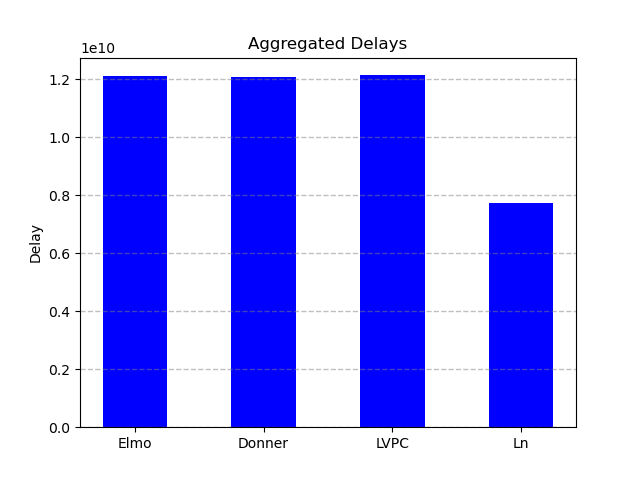
\includegraphics[width=\textwidth]{../simulation/Delays_power_law.png}
  \end{subfigure}
  \begin{subfigure}{.3293\textwidth}
  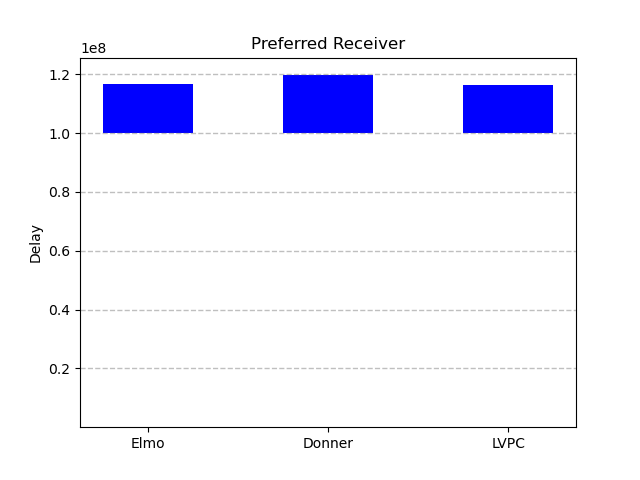
\includegraphics[width=\textwidth]{../simulation/Delays_preferred_receiver.png}
  \end{subfigure}
  \begin{subfigure}{.3293\textwidth}
  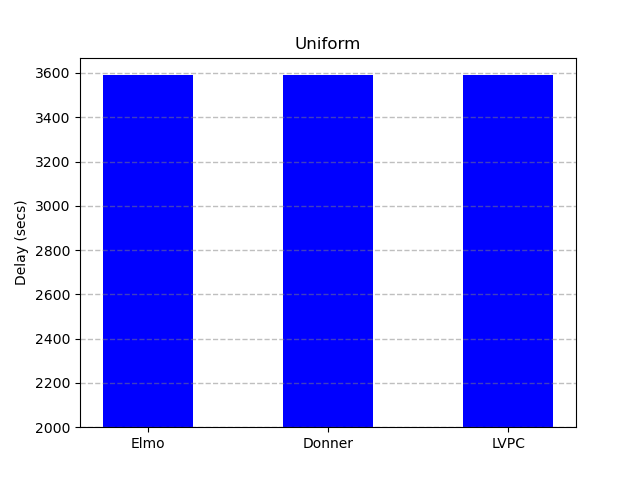
\includegraphics[width=\textwidth]{../simulation/Delays_uniform.png}
  \end{subfigure}
  \caption{Average per-payment delay in seconds. Less is better.}
  \label{graph:delays}
  \end{figure}
  \begin{figure}
  \begin{subfigure}{.3293\textwidth}
  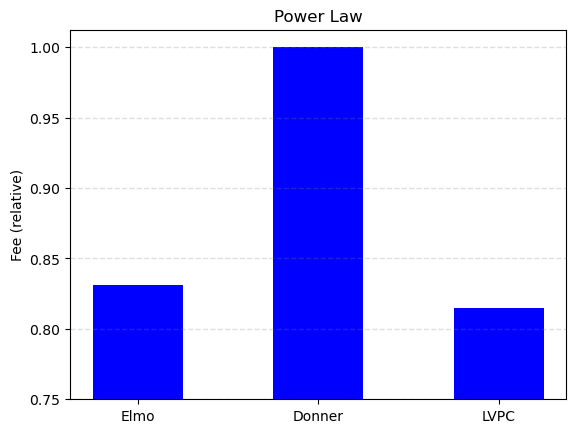
\includegraphics[width=\textwidth]{../simulation/Fees_power_law.png}
  \end{subfigure}
  \begin{subfigure}{.3293\textwidth}
  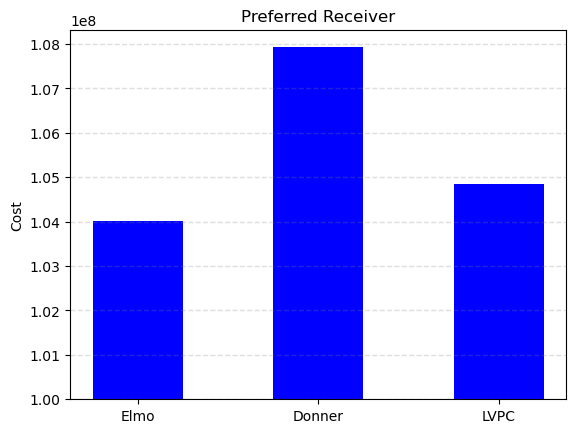
\includegraphics[width=\textwidth]{../simulation/Fees_preferred_receiver.png}
  \end{subfigure}
  \begin{subfigure}{.3293\textwidth}
  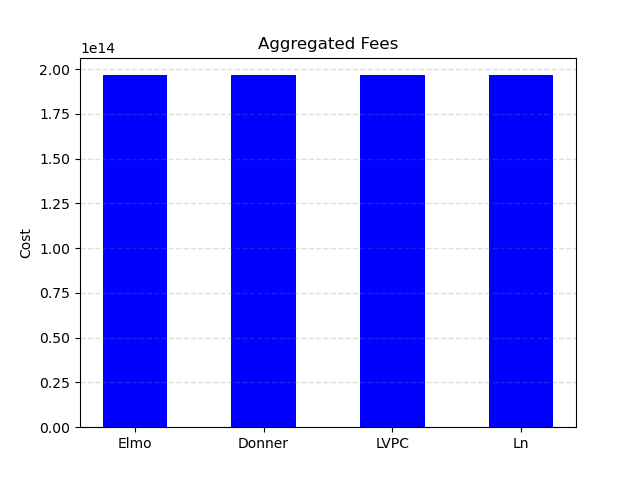
\includegraphics[width=\textwidth]{../simulation/Fees_uniform.png}
  \end{subfigure}
  \caption{Average per-payment relative fee. Less is better.}
  \label{graph:fees}
  \end{figure}
  \addtolength{\intextsep}{15pt}
